\section{Results}\locallabel{sec:results}

In this section, we present the results of using Hairball to assist in
determining the level of competence demonstrated by students' \sprogram{s} for
several computer science concepts. For each concept, we will compare the labels
Hairball assigned to instances of the concept with those assigned via manual
analysis. We will use the second manual analysis as the ground truth, and look
at both the false positive and the false negative rates for Hairball and the
manual analysis. Although our results include the labels \semincor{}, \incor{},
and \incom{} to demonstrate that Hairball can be used for more than binary
labeling, our assessment focuses on instances that are either labeled
\correct{} or not. Thus, we consider a false positive to be an instance that
was labeled \correct{}, when in fact it is not, and a false negative to be an
instance that is actually \correct{}, but was not labeled as such. For manual
analysis both false positives and false negatives represent the inaccuracies of
manual assessment. For Hairball, false negatives can be considered warnings,
i.e., they are used to indicate the need for additional manual
analysis. However, any false positives produced by Hairball are cause for
concern.


\subsection{Initialization}
\begin{figure}[!t]
\centering
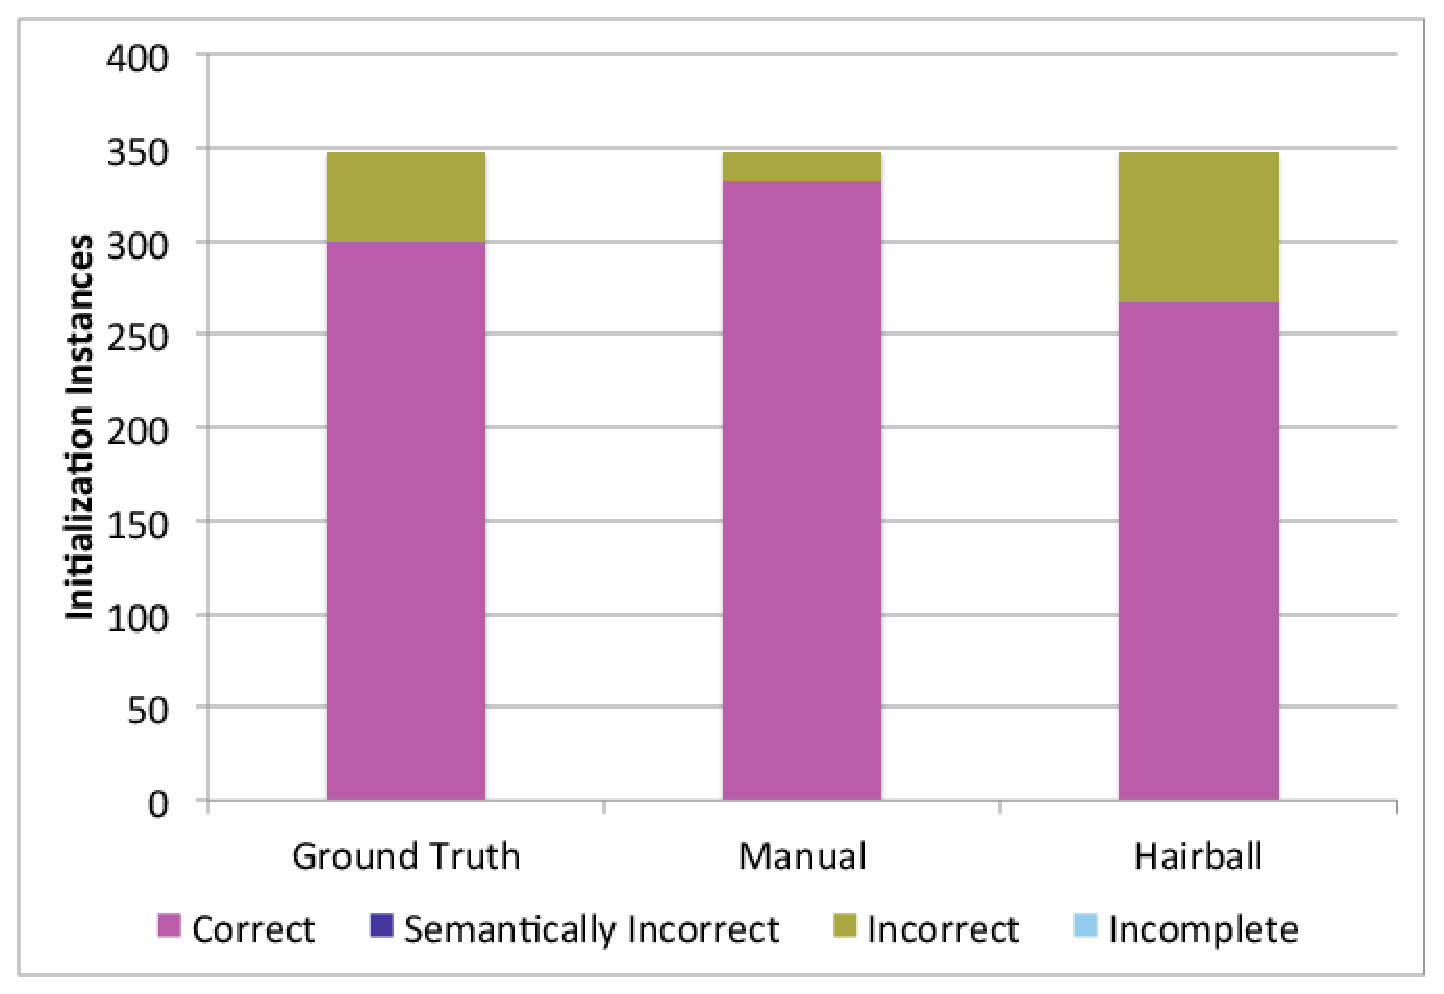
\includegraphics[trim=.3in .15in .3in .15in, clip,
  width=5.25in]{graphs/AutoInit.eps}
\caption{Compares the initialization instance labels. Note that this analysis
  used only the \correct{} and \incor{} labels. Manual analysis resulted in
  thirty-two false positives, and Hairball resulted in thirty-three false
  negatives.}
\locallabel{fig:initialization}
\end{figure}

We begin with initialization. Recall from Section~\localref{sec:plugins} that
Hairball looks for attributes that are modified, and expects to find a
corresponding \abs{} block in the \initzone{} in order to consider an instance
\correct{}. The manual analysis, on the other hand, only involved running the
\sprogram{} twice, and confirming that the two executions matched.

Figure~\localref{fig:initialization} provides the classification of the 348
initialization instances discovered across the fifty-eight \sprogram{s}. Of the
sixty-five instances that Hairball and the manual analysis labeled differently,
Hairball was accurate for thirty-two of the instances. Many of the remaining
thirty-three instances were not possible for Hairball to label as \correct{}
due to initialization taking place outside of the \initzone{}. For example, an
initially hidden sprite can correctly have its position initialized just before
the sprite becomes visible. In spite of this discrepancy, these results overall
indicate that Hairball is successful at pointing out problems in
initialization.

\subsection{Say and Sound Synchronization}
\begin{figure}[!t]
\centering
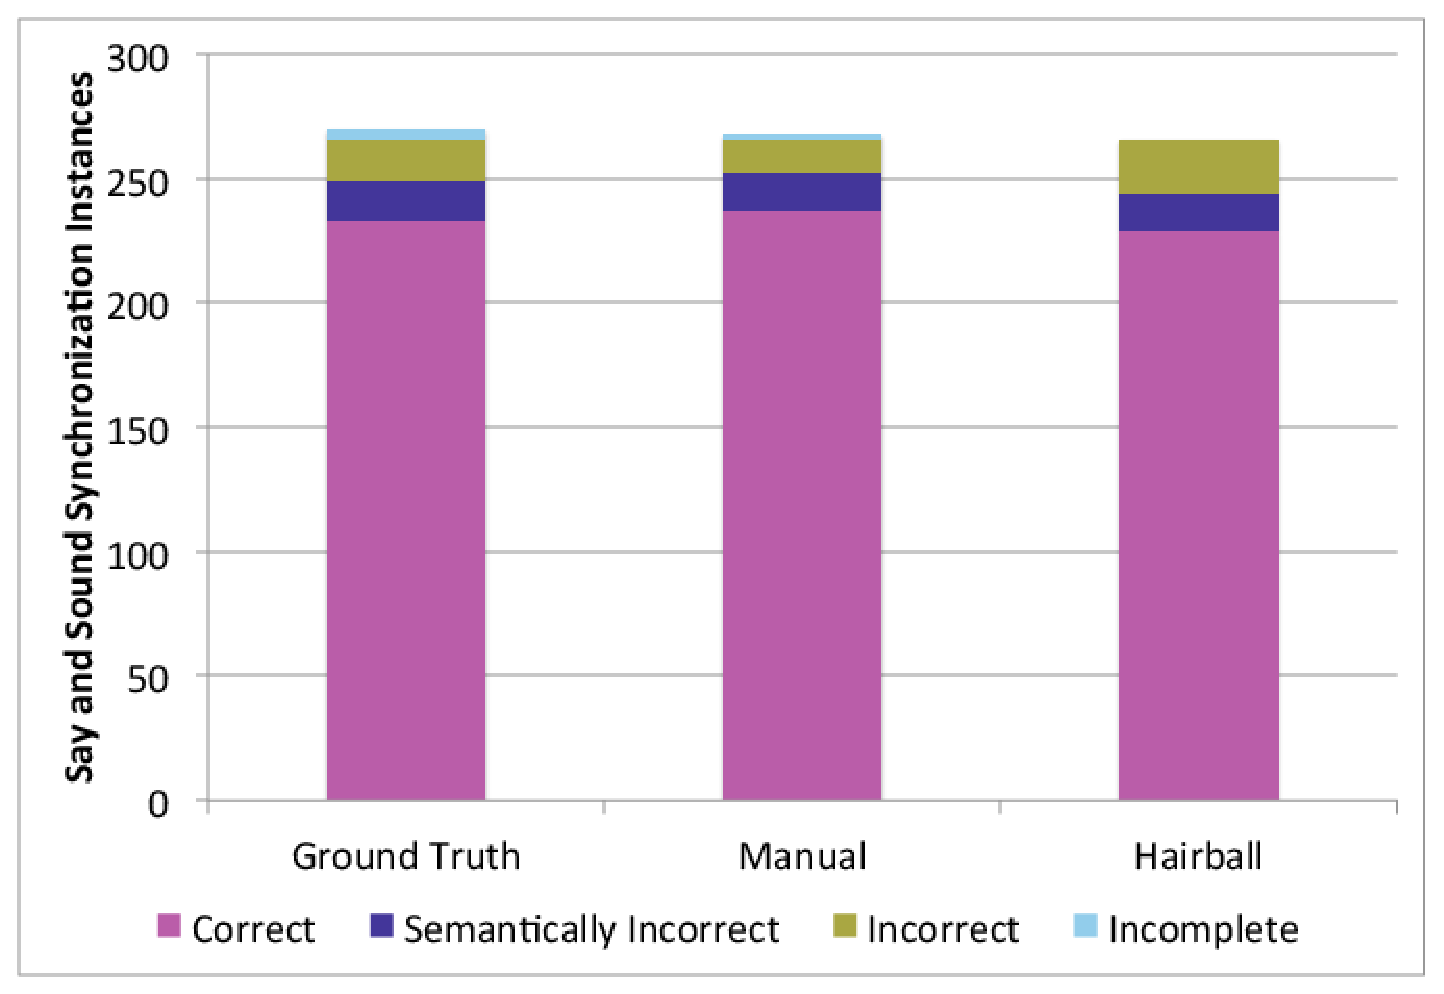
\includegraphics[trim=.3in .15in .3in .15in, clip,
  width=5.25in]{graphs/AutoSaySoundSync.eps}
\caption{Compares the say and sound synchronization instance labels. Manual
  analysis and Hairball failed to detect two and four instances respectively
  and manual analysis resulted in four false positives.}
\locallabel{fig:saysoundsync}
\end{figure}


Figure~\localref{fig:saysoundsync} shows the results of identifying and
labeling instances of synchronization between speech bubbles and sound
files. Manual analysis identified 237 \correct{} instances, and a total of
thirty-one other instances. Hairball identified 229 \correct{} instances and
thirty-seven others. Manual analysis and Hairball failed to find two and four
instances respectively.

Comparison with the ground truth results in four false positives for manual
analysis. Hairball labeled its instances with 100\% accuracy. Two of the four
instances undetected by Hairball were labeled \incom{} by manual
analysis. Hairball failed to detect these instances due to a separation of the
\say{} and \playsound{} blocks with a \broadcast{} block. To detect such
instances, Hairball would need to additionally inspect all scripts triggered by
the broadcast event to ensure none of them interfered with either the display
of the speech bubble or the playing of the sound file.

\subsection{Broadcast and Receive}
\begin{figure}[!t]
\centering
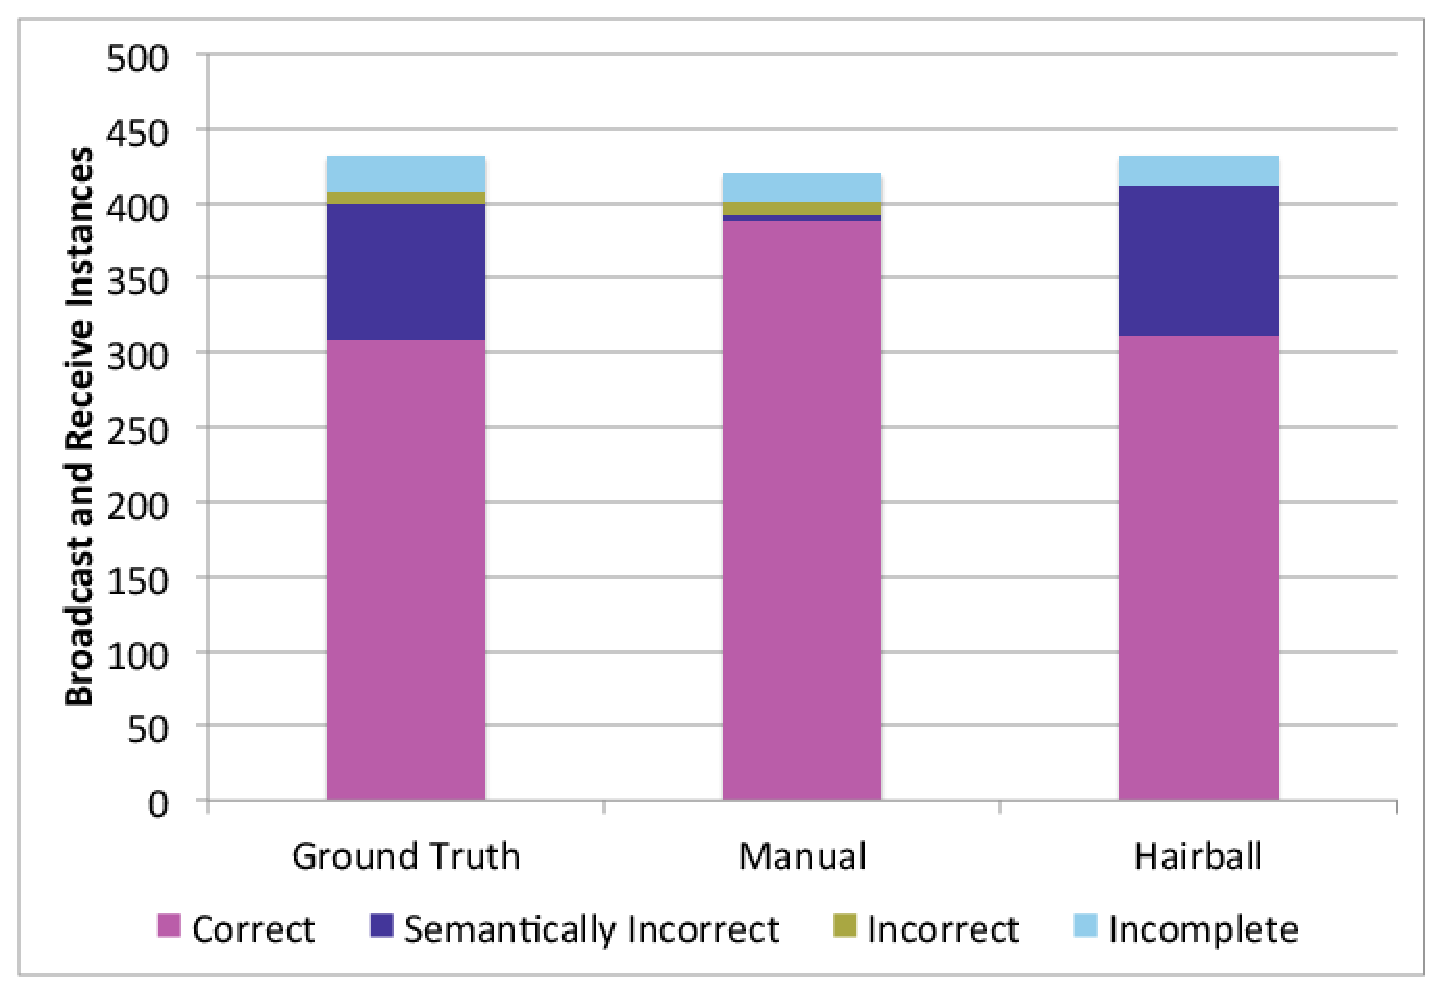
\includegraphics[trim=.3in .15in .3in .15in, clip,
  width=5.25in]{graphs/AutoBroadcastReceive.eps}
\caption{Compares the broadcast and receive instance labels. Manual analysis
  failed to discover twelve instances, and resulted in seventy-nine false
  positives. Hairball detected 100\% of the instances with three false
  positives.}
\locallabel{fig:broadcastreceive}
\end{figure}

Figure~\localref{fig:broadcastreceive} shows the results of detecting and
labeling instances of broadcast and receive. Here, the manual analysis differed
from Hairball by additionally verifying that the intended action is performed
for \correct{} instances. Hairball is limited to static analysis, thus it is
unable to perform this additional step.

Overall, manual analysis failed to discover twelve instances, and identified
388 \correct{} instances, of which, seventy-nine were false positives. Hairball
discovered 100\% of the instances with zero false negatives. However, three of
the 312 instances Hairball labeled as \correct{} were false positives. Although
these three instances represent \correct{} usage of the \broadcast{} and
\receive{} blocks, the ground truth analysis determined the evaluation behavior
to be \incor{}.



\subsection{Complex Animation}

\begin{figure}[!t]
\centering 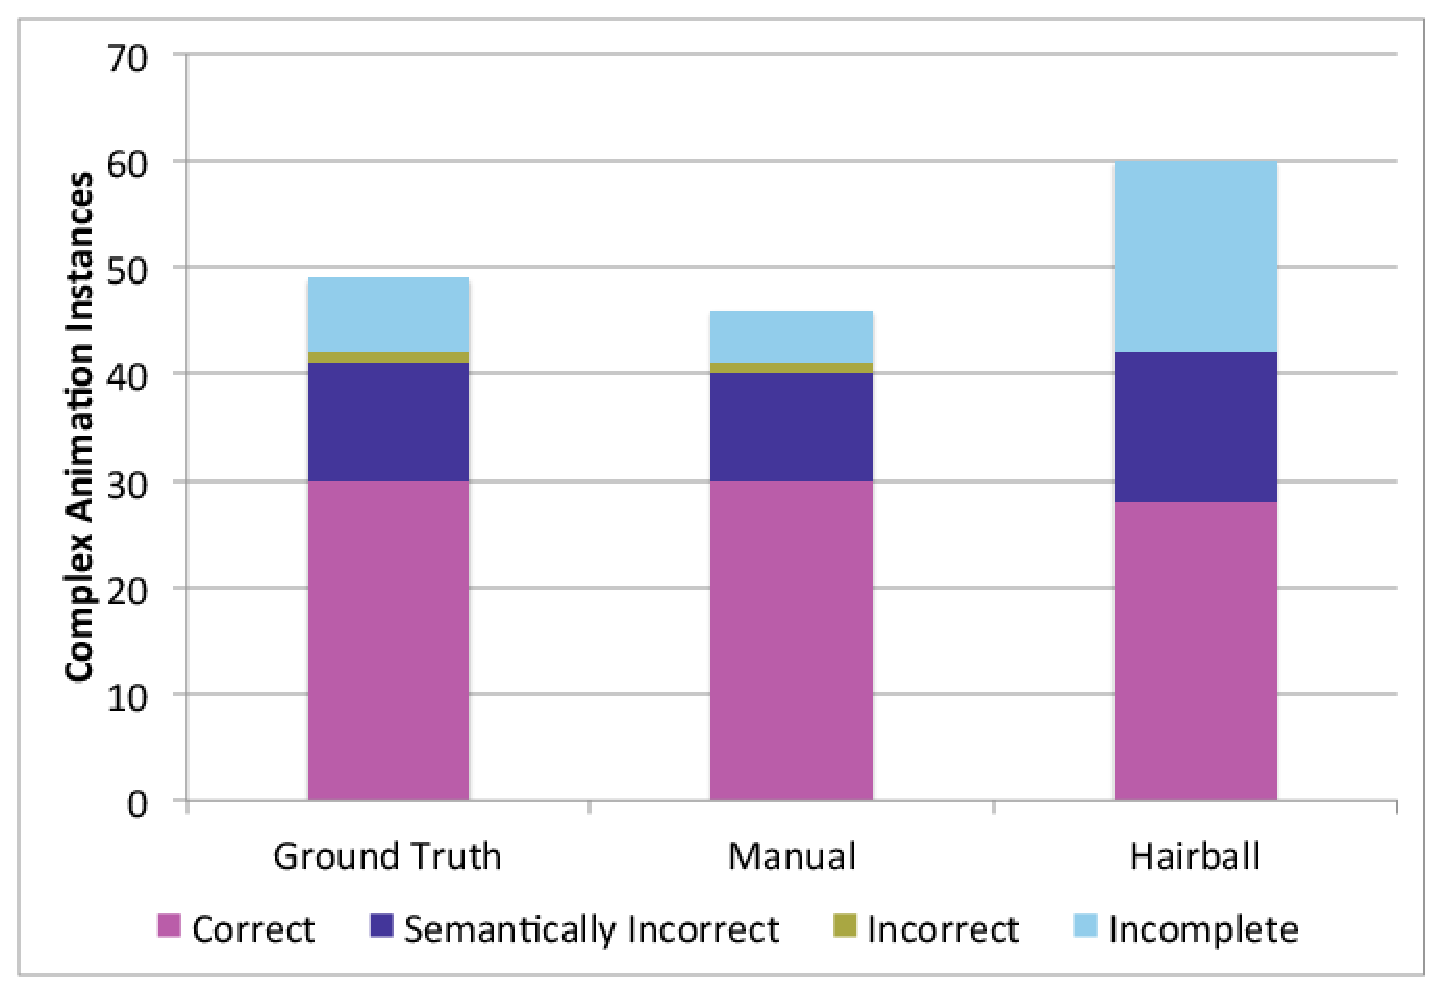
\includegraphics[trim=.3in .15in .3in .15in, clip,
  width=5.25in]{graphs/AutoAnimation.eps}
\caption{Compares the complex animation instance labels. Manual analysis failed
  to detect three instances whereas Hairball found eleven items that were
  determined to not be instances of complex animation. Hairball resulted in two
  false negatives.}
\locallabel{fig:animation}
\end{figure}

Complex animation was especially difficult for Hairball to detect.  As
Figure~\localref{fig:animation} shows, manual analysis was 100\% accurate at
labeling the forty-six instances found, and only failed to detect three
instances. Hairball, on the other hand, labeled eleven items as \incom{} that
the ground truth analysis determined to not be instances at all. Excluding
these instances, Hairball identified twenty-eight \correct{} instances, and
twenty-one others with only two false negatives.

Hairball identified too many instances of complex animation due to the
subjective nature of what is considered an animation.  For example, Hairball
detects an animation according to where the loops and repetition are
located. Several times, Hairball detected two separate animations, when manual
analysis determined that those two actions were working together to create a
single larger animation. Additionally, Hairball considered a move, wait, and
change in appearance as an \incom{} animation instance. In such cases, manual
analysis recorded nothing.

\subsubsection{Summary Results}
\begin{figure}[!t]
\centering 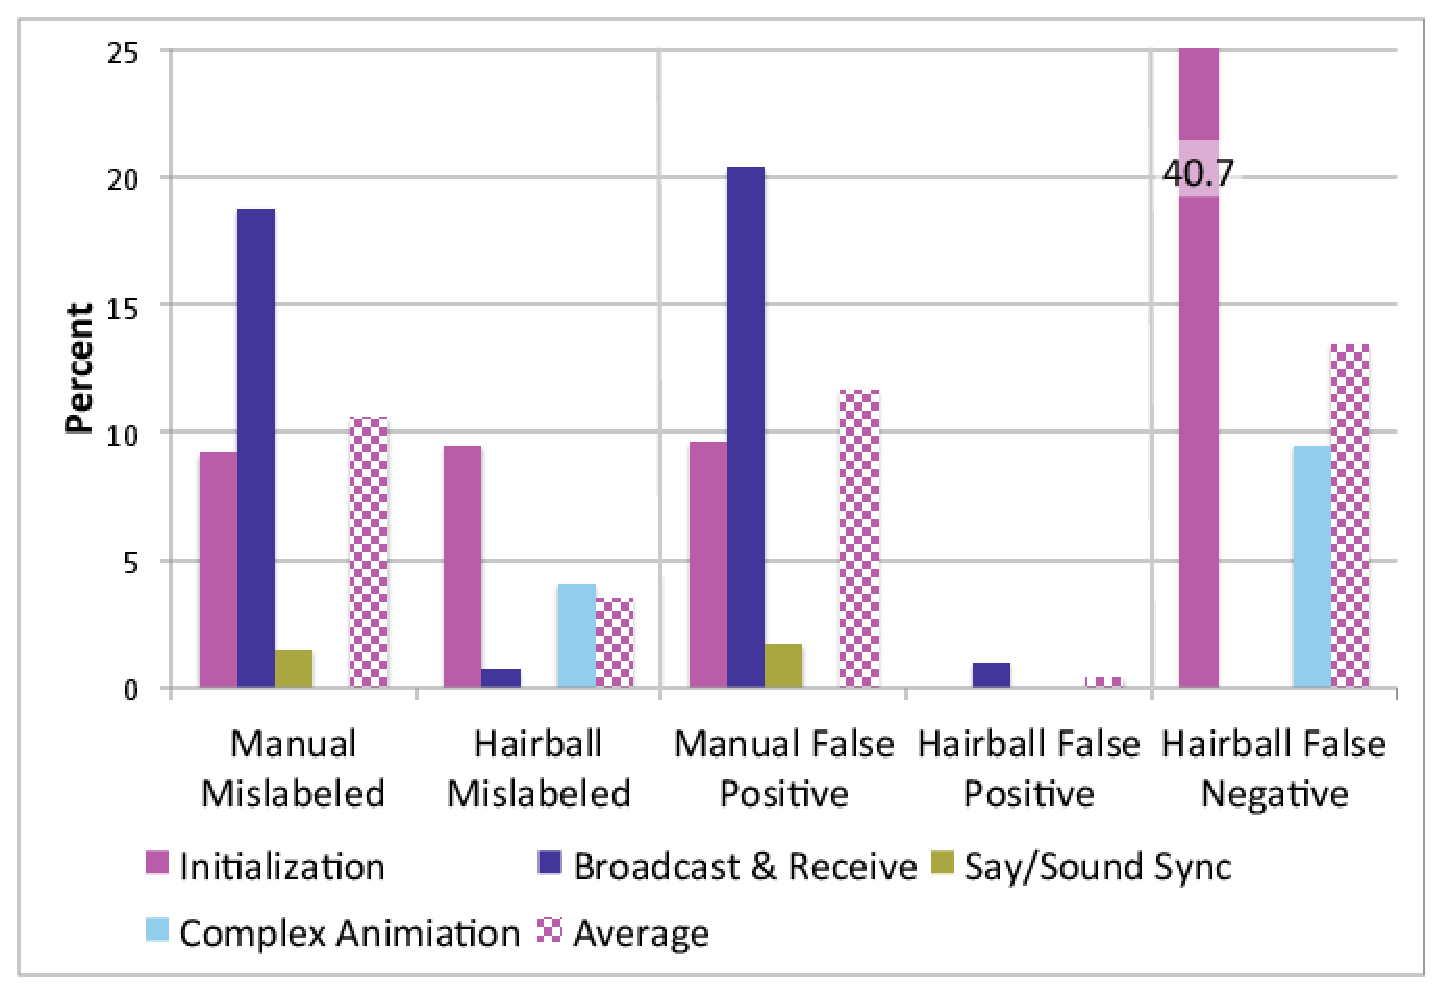
\includegraphics[trim=.3in .15in .2in .15in, clip,
  width=5.25in]{graphs/AutoSummary.eps}
\caption{Provides a summary of the percent of mislabeled, false positive, and
  false negative instances resulting from manual analysis and Hairball for each
  of the four computer science concepts and the average. The \emph{Manual False
    Negative} category was omitted as manual analysis resulted in zero false
  negatives. The y-axis is truncated for the smaller values, thus the tallest
  bar should extend to 40.7\%. Missing bars represent 0\%.}
\locallabel{fig:summary}
\end{figure}

Figure~\localref{fig:summary} shows three sets of results across all four
computer science concepts and the overall average. The first is the mislabel
rate of manual analysis and Hairball. Percentages closer to zero indicate
higher accuracy. We see that Hairball is actually slightly more accurate
overall than manual analysis; largely due to Hairball's accuracy in labeling
broadcast and receive instances.

The second set of results is the rate of false positives. Manual analysis's
overall false positive rate of 11.7\% indicates that manual analysis is quite
error prone. On the other hand, Hairball's false positive rate of 0.4\%
strongly indicates Hairball is accurate at labeling \correct{} instances.

Finally, the third set of results is the rate of false negatives. The lack of
false negatives for manual analysis makes sense, considering Hairball was
created according to the first manual analysis. Although Hairball has an
overall false negative rate of 13.5\%, we believe this rate to be acceptable
due to the fact that four out of five instances in our ground truth set were
labeled \correct{}, meaning the use of Hairball on a similar corpus of
\sprogram{s} would reduce the set of instances requiring manual analysis by
80\%.
